% this file is called up by thesis.tex
% content in this file will be fed into the main document

%: ----------------------- name of chapter  -------------------------
\chapter{Conducting Experiments} % top level followed by section, subsection
\label{chapterCondExp}

%: ----------------------- paths to graphics ------------------------

% change according to folder and file names
\ifpdf
    \graphicspath{{X/figures/PNG/}{X/figures/PDF/}{X/figures/}}
\else
    \graphicspath{{X/figures/EPS/}{X/figures/}}
\fi

%: ----------------------- contents from here ------------------------

This chapter gives an outline of the process of conducting cycle- and application-level experiments that are described in the previous chapter. It provides a detailed description of what needs to be done to run the described experiments on the Xeon 5130 and Xeon E5-2695 v2 processors. If a reader wishes to replicate the study, the content of this chapter will give a detailed description on how to do that. It starts from giving a description of the hardware that was used in the project. It also lists main constraints that had to be faced while running the experiments.

\section{Hardware}
\label{sec_hardware}

The faculty of Computer Science in the National University of Ireland, Maynooth provided access to a machine powered by one Intel Xeon 5130 dual-core processor. Rights to SSH into the computer and use it for this research were also given. Additionally, the Ireland's High-Performance Computing Centre (ICHEC)\footnote{\url{https://www.ichec.ie/}} offered to create an account on their fionn3 server. That server has 320 nodes (7680 cores; 20 TiB RAM) and each node contains 24 (2x12) Ivy Bridge CPU cores that are powered by Intel Xeon E5-2695 v2 CPUs. Fundamentally, the processors utilised in the machines are similar, but they exhibit different levels of support to varies technologies. For example, the Xeon E5-2695 v2 supports the \textit{RDTSCP} instruction, and the Xeon 5130 does not. Moreover, Intel Xeon 5130 is 7 years older than Intel Xeon E5-2695 v2 and they have a number of vital differences. Such differences are beneficial for the analysis of results obtained in the project. A table \ref{xeonTable} outlines main characteristics of both machines.

\begin{table*}
\caption{Description of the processors used in the study}
\centering 
\begin{tabular}{lll}
\hline
                & \textbf{Intel Xeon 5130 (NUIM)} & \textbf{Intel Xeon E5-2695 v2 (ICHEC)} \\ \hline
Server          & IBM System x3550 -[797841Y]-                     & Fionn\footnote{\url{https://www.ichec.ie/infrastructure/fionn}}                       \\
Launch year     & 2006                       & 2013                             \\
Lithography     & 65 nm                      & 22 nm                            \\
Number of cores & 4                          & 24                               \\
Clock speed     & 2 GHz                      & 2.4 GHz                          \\
L1 cache size   & 32 KB                      & 32 KB                            \\
L2 cache size   & 4 MB                    & 256 KB                           \\
L3 cache size   & None                       & 30 MB \\
Cache line size   & 64 B                       & 64 B \\
Linux version   & 3.2.0-4-rt-amd64           & 3.0.74-0.6.6-default
\end{tabular}
\label{xeonTable}
\end{table*}

No CPU-specific specification for both processors used in the study (e.g. cache latency times) is available from Intel. The publicly-available software developer manual (especially chapter 11 in that document) was used for reference \cite{Intel2014}. Through experimentation and referring to a resource that discusses CPUs from the Intel Xeon 5600 processor family with a similar to what is used in the study architecture \cite{Balakrishnan2010}, layout diagrams were produced for both the Xeon 5130 and the Xeon E5-2695 v2. The figure \ref{Threads_cpu_diagram} outlines the design of the Intel Xeon 5130 processor. This is a multi-chip processor that has two CPUs. All cores have private Level 1 caches, all chips have private Level 2 caches. This processor does not have a shared Level 3 cache. Two chips are connected by a QPI (QuickPath Interconnect) point-to-point processor interconnect bus \cite{Intel2009a}.

\begin{figure}[ht!]
\centering
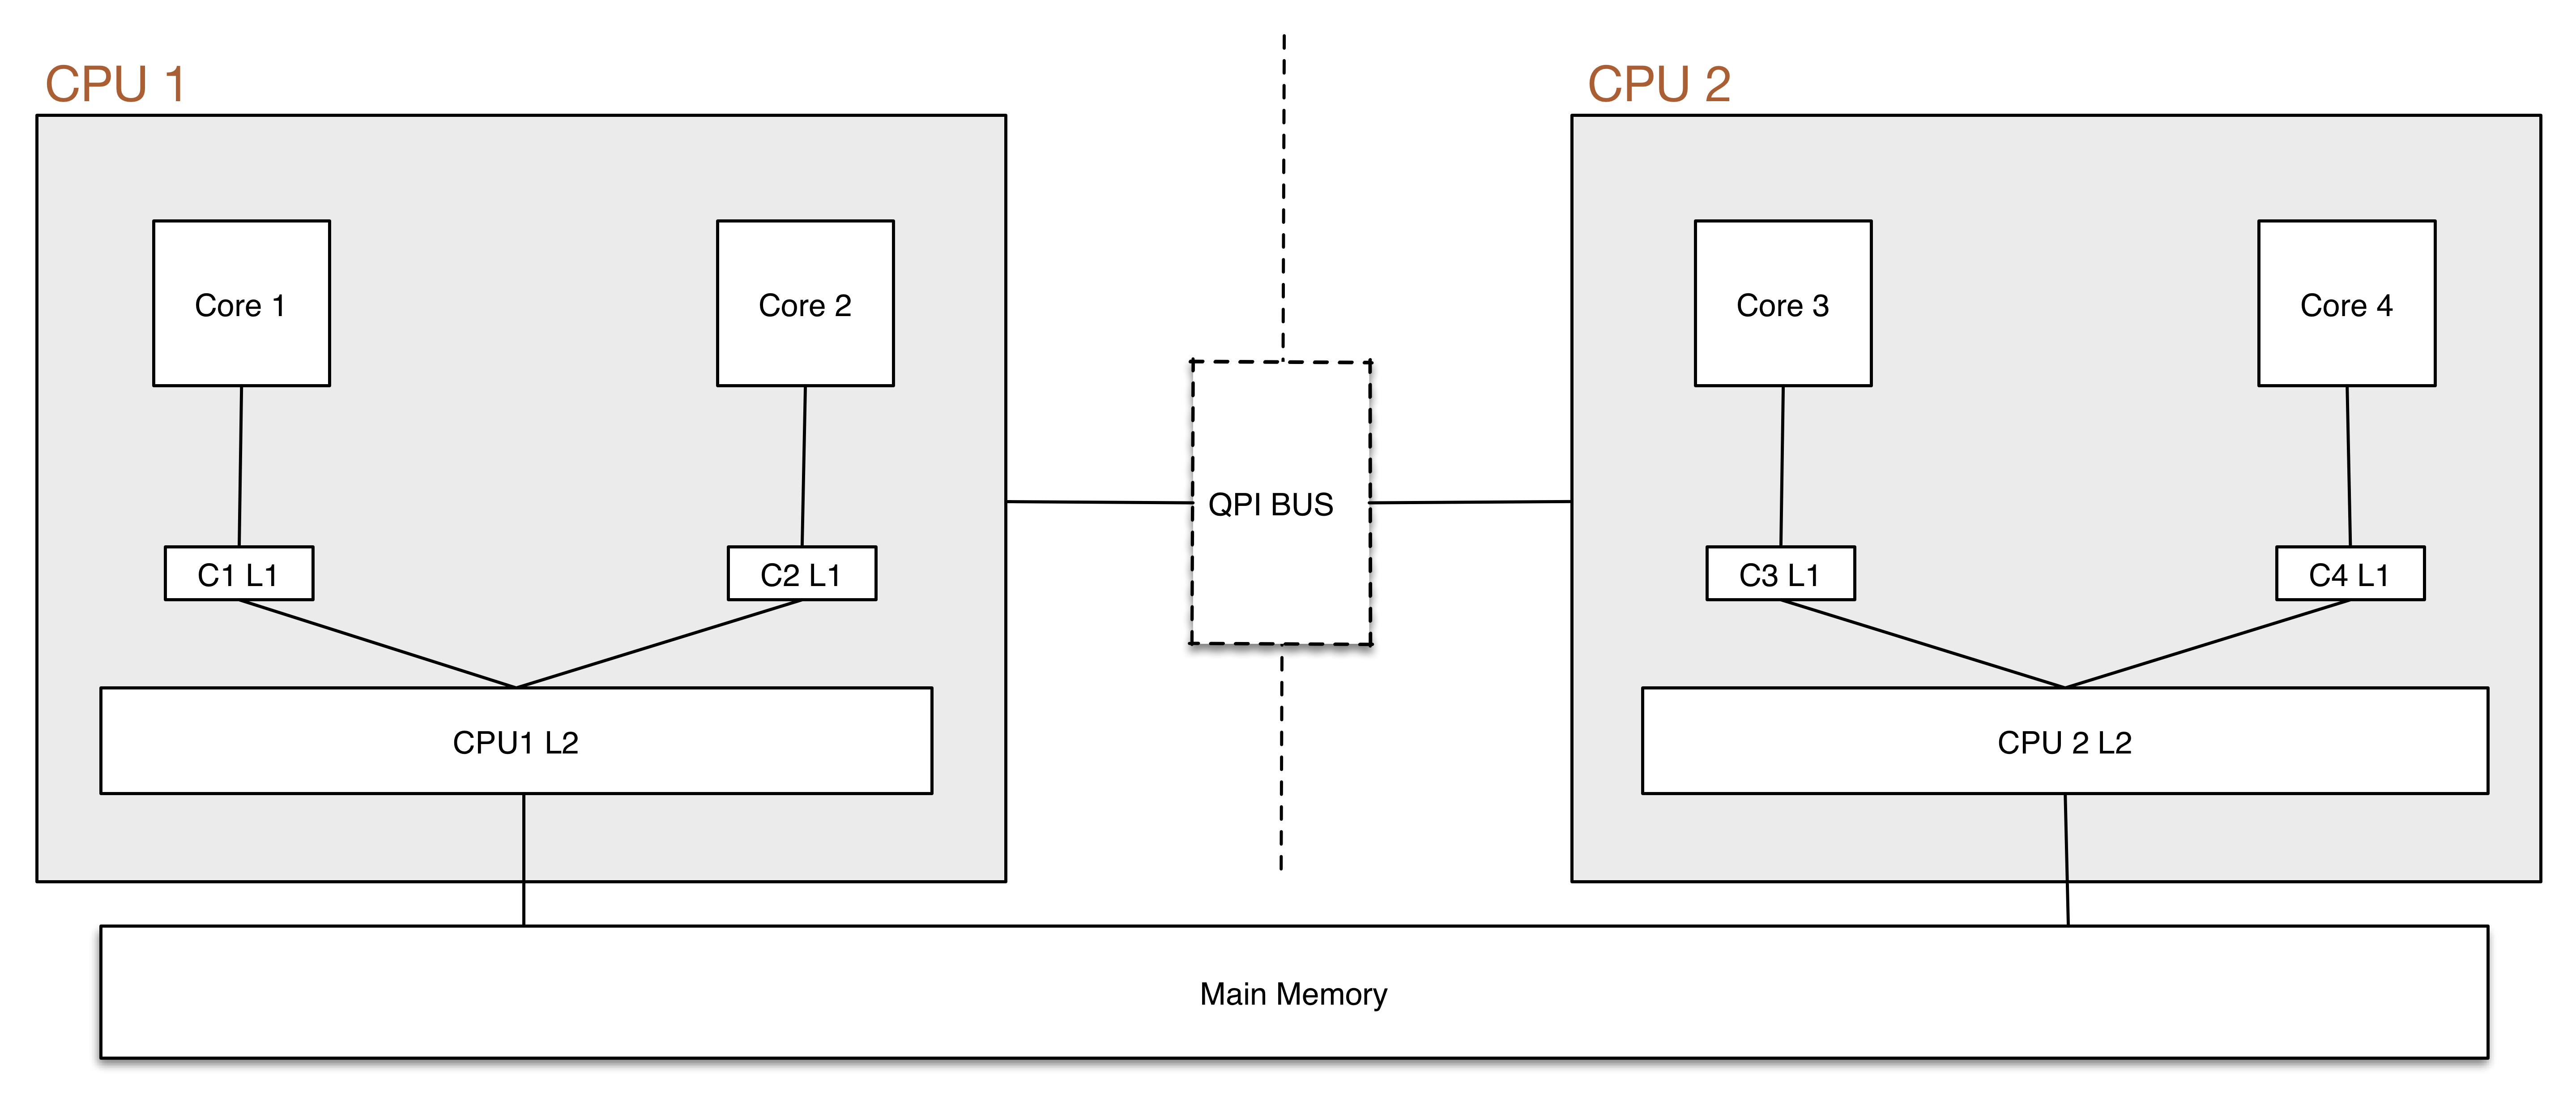
\includegraphics[width=145mm]{4/Xeon_5130.png}
\caption{Diagram of the layout of Xeon 5130}
\label{layout_xeon_5130}
\end{figure}

The diagram \ref{layout_xeon_2695} represents all main components of the Intel Xeon E5-2695 v2 CPU. This CPU has 24 cores, each core has private L1 and L2 caches, each of two dies has a rather big 30 MB L3 cache. The cores of this processor are also connected by a QPI bus.

In both cases the write-through (WT) cache is considered. Obtaining the exact figures for latency and throughput of different caches that are used in these processors, that can be supported by a published resource, proved to be impossible. The only official document from Intel \cite{Levinthal} that could be found reports latency for the processor Core i7 and the processor family Xeon 5500. The Xeon 5500 CPU is relatively similar to the Xeon 5130, yet it is three years newer and it works on much higher frequencies and instead of two cores it includes up to four hyper-threaded cores \cite{Intel2009}. The cache itself is fundamentally different, as processors of that type have Intel® Smart Cache-enabled caches \cite{Intel2012}.

\begin{figure}[ht!]
\centering
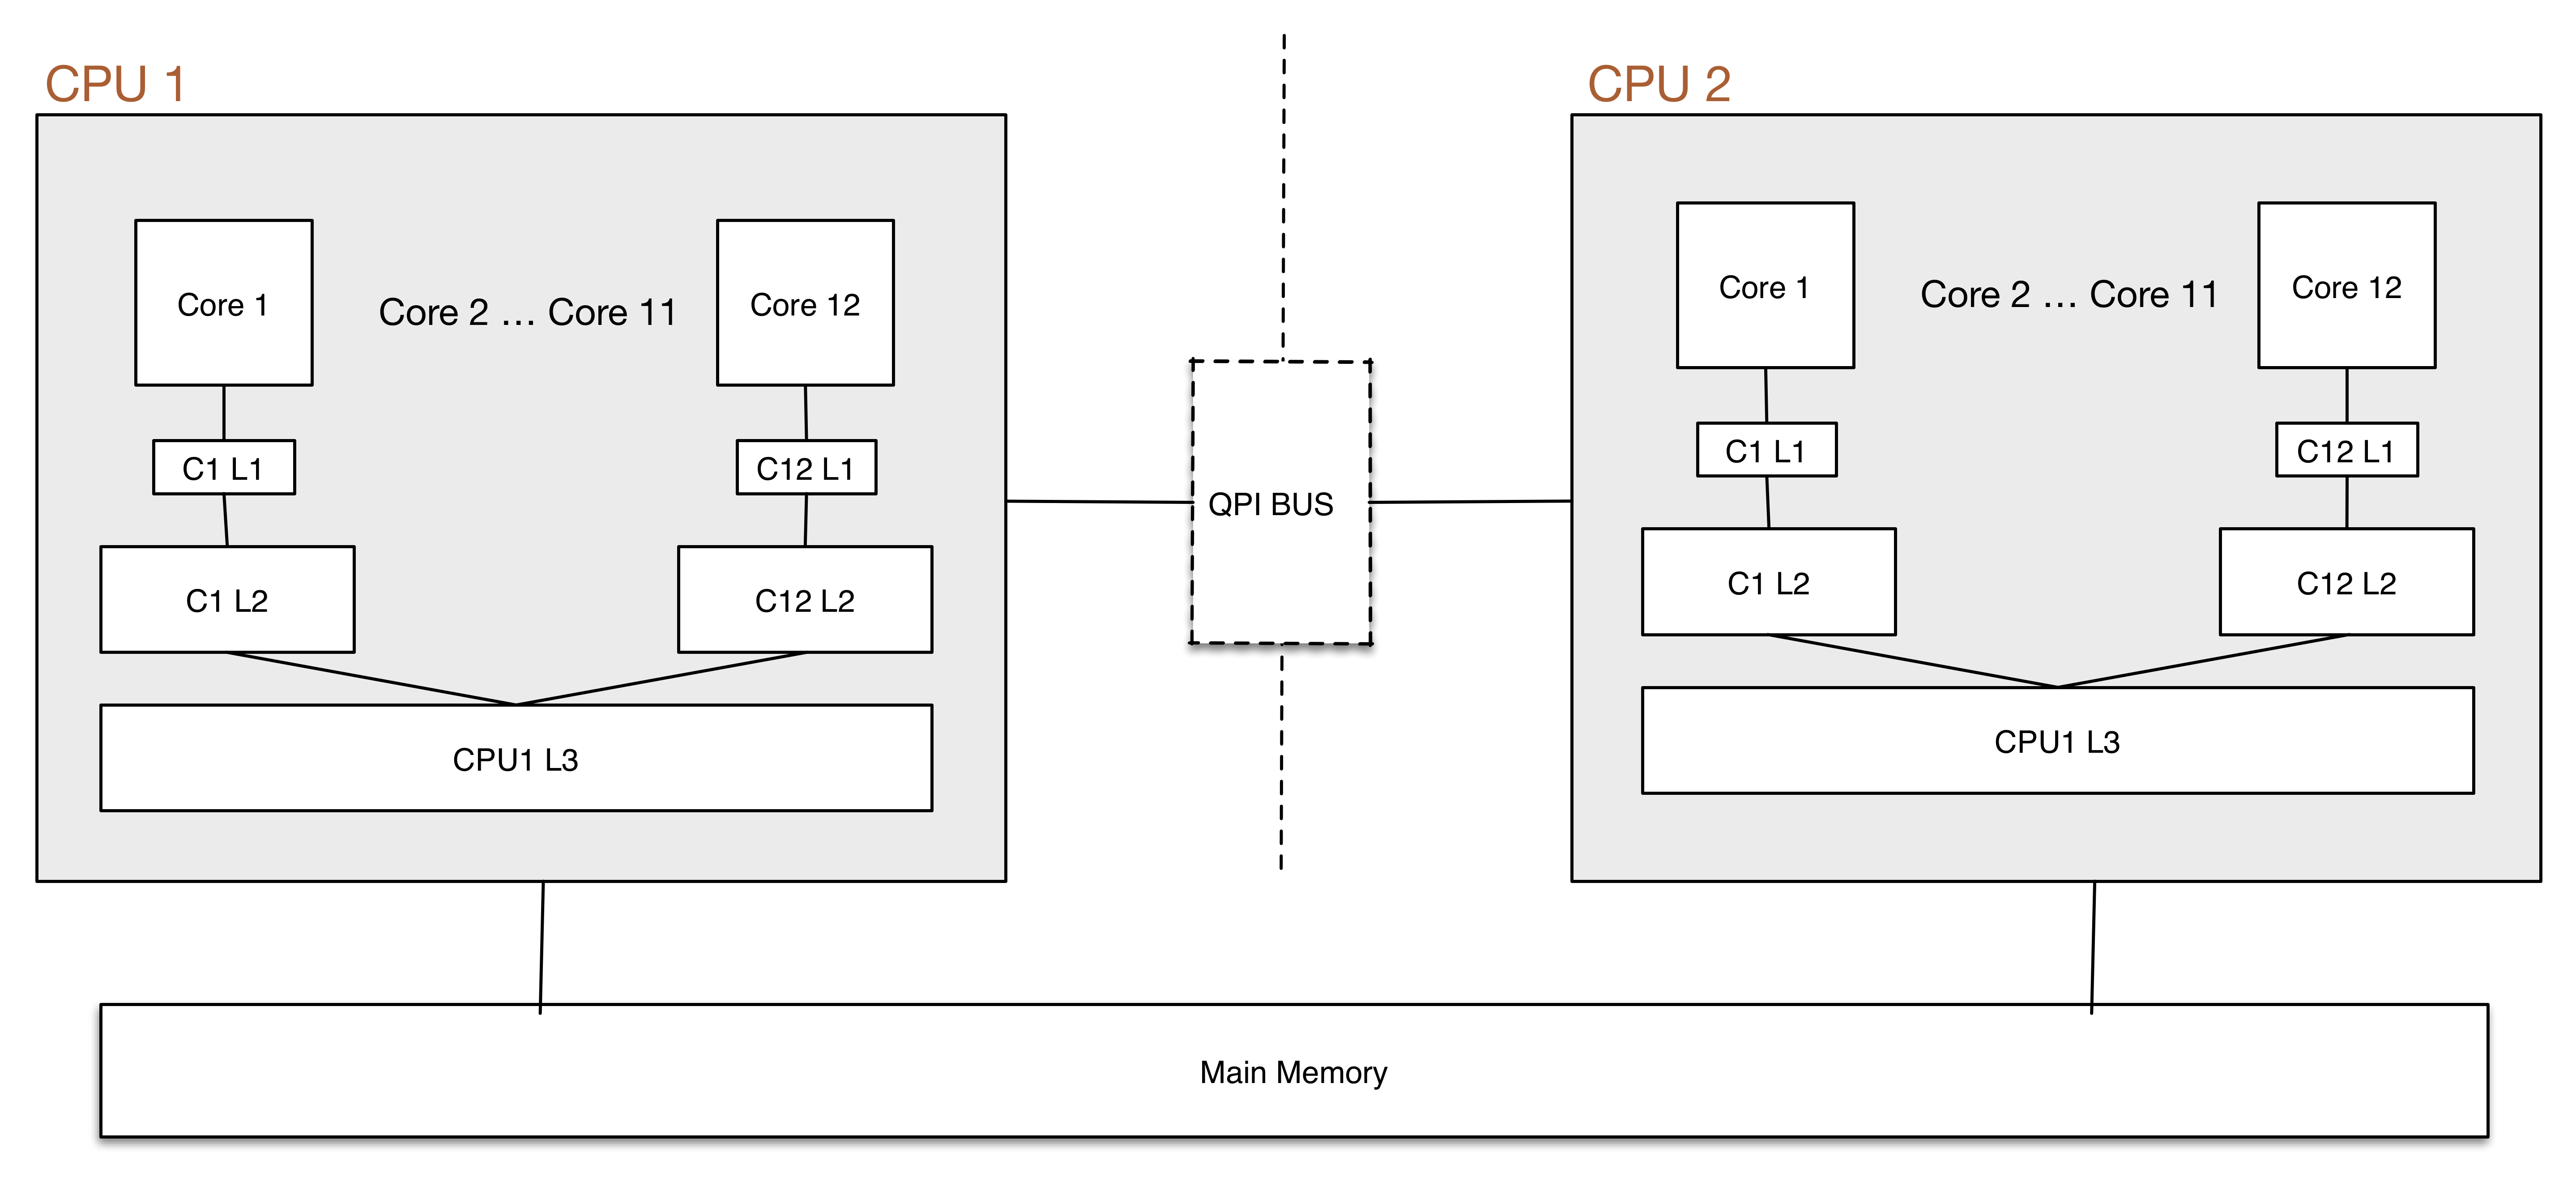
\includegraphics[width=145mm]{4/Xeon_E5-2695_v2.png}
\caption{Diagram of the layout of Xeon E5-2695 v2}
\label{layout_xeon_2695}
\end{figure}

The machine powered by Xeon 5130 consists of a single node, but the ICHEC's server is a workstation that consists of a number of units of computation. To be able to run the designed experiments, all tests had to be run on a single node. The experiments are relatively small, so any noticeable advantages could not be achieved by running experiments on multiple nodes. Both the Xeon 5130 and the Xeon E5-2695 v2 support the Intel® Hyper-Threading Technology (Intel® HT Technology) that allows an execution core to function as two logical processors. This technology was disabled on the Xeon 5130 to improve accuracy of achieved results. Disabling this feature could not be requested on the Xeon E5-2695 v2, although it is speculated that is is disabled by default.

\section{Constraints}
The designed experiments are constrained by a number of factors. Accuracy of results depends on isolation of processes/threads that belong to the run experiment and ability to terminate as many unnecessary processes as possible. Experiments are run from a Linux terminal, which allows to eliminate overhead caused by a GUI and other supporting system tasks, but the commands are executed with SSH that imposes additional overhead. The experiments are executed on hardware that was provided by the hosting university, access to more sophisticated and advanced machines could not be granted due to financial and bureaucratic reasons. All of these constraints were considered during the stage of designing the experimental environment and the experiments.

\section{Experiments}

A series of experiments were designed in the scope of the project. They are described in section \ref{experimentsDesign}. This section outlines how they can be run in the developed experimental environment and how results can be collected.

\subsection{Running Experiments on Servers}

All experiments were run from the terminal window on Mac OS X Mavericks. Both machines could be accessed by using the SSH protocol. Refer to figure \ref{terminal-nuim} for an image of the Terminal window with typed in commands that are required to SSH into the Xeon 5130, enter the directory with the source code of the experimental environment and the experiments, compile the code and run it. One may observe a \textit{make} command used to run the experiments. A makefile was created to optimise the process of running required experiments. Refer to appendix \ref{app:listingMakefile} for a source code of the file. This makefile can be used on both Linux-based Operating Systems and on Mac OS.

\begin{figure}[ht!]
\centering
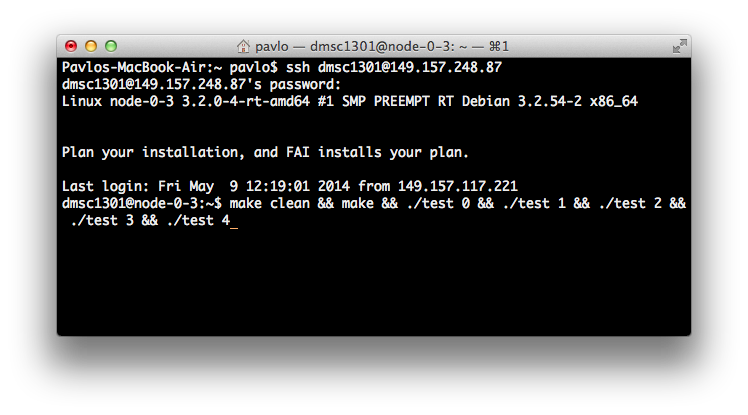
\includegraphics[width=145mm]{5/terminal-nuim.png}
\caption{Commands required to SSH into the Xeon 5130 and run the experiments}
\label{terminal-nuim}
\end{figure}

In case of the Xeon E5-2695 v2, since that machine has multiple nodes, the experiments had to be scheduled to be run on a single node. Refer to the Listing \ref{lst:ichecCommand} for the exact command used to schedule a job. This command was derived after reading documentation available at \cite{ICHEC2014a}. The \textit{qsub} command is utilised to explicitly send a job to a given queue. The argument \textit{-A nuim01} defines the account string associated with the job. Then, the argument \textit{-l nodes=1:ppn=24} specifies the resources that are required by the job, in this case one node and 24 units of computation associated with the node are asked. The \textit{walltime=0:29:00} mentiones the maximum amount of time that the job can be run for, in this case it says that the job can be run for the maximum of 29 minutes. Lastly, the argument \textit{-I} means that the new session needs to be interactive (with access to issuing new commands via the command prompt).
              
\begin{lstlisting}[
language=bash,
caption={Command to schedule a job on one node in the Xeon E5-2695 v2},
label={lst:ichecCommand}
]
qsub -A nuim01 -l nodes=1:ppn=24 walltime=0:29:00 -I
\end{lstlisting}

Files with source code can be copied onto the servers and back by the secure copy command \textit{scp}. Measured data can then be analysed on the local machine.

\subsection{Execution of Experiments}

When the experimental environment is compiled, the experiments are ready to be run. All experiments could be executing by running the compiled experimental environment and passing a single argument: a ID of an experiment. For example, a command \textit{./test 2} will run the Experiment 2. When experiments are executed, different information may be outputted. A level of details in the information shown to a user may be configured by defining variables \textit{DEBUG} and \textit{DETAILED\_DEBUG} (by default defined in the \textit{conf.h}\footnote{\url{https://github.com/Hollgam/Impact-of-cache-on-multi-threaded-programmes/blob/master/test/
src/conf.h}} file). If a variable \textit{SHOW\_RESULTS} is defined, the summary of results from running the experiments is also outputted onto the screen. 

To continue, the experimental environment could not be prepared to support completely free from the impact of the Operating System experiments. It was decided to produce two CSV files for each experiment. One file with filtered data and another one with unfiltered data. Files are named as \textit{``CPU\_TYPE-EXPERIMENT-RUN.csv"}, where \textit{CPU} indicates a type of CPU that an experiment was run on (e.g. ``xeon"), \textit{TYPE} shows the type of data stored in the file (can be either ``clean" for filtered data or ``dirty" for unfiltered data), \textit{EXPERIMENT} gives the ID of the experiment, and \textit{RUN} shows a run of the experiment (if an experiment is run more than once, individual CSV files are generated for each run). All files are placed in a \textit{results} folder. They present quantitative information gathered before and after running experiments and mention numbers of any interrupts and minor and major page faults detected while executing the experiments. Files with filtered data contain timing results only from running those experiments that were not interrupted by interrupts or page faults, i.e. if such unwanted processes were detected during execution of all runs of an experiment, its duration is noted as ``0".

\begin{table*}
\caption{A sample of a CSV file with filtered data}
\centering 
\scalebox{0.8}{
    \begin{tabular}{lllllllllll}
    N         & Time   & TimeMin   & 1.INT & 1.PFMIN & 1.PFMAJ & 2.INT & ... & 10.INT & 10.PFMIN & 10.PFMAJ \\
    0         & 581742 & 581742 & 0     & 6       & 0       & 0     & ... & 0      & 2        & 0        \\
    8         & 591849 & 581742 & 0     & 0       & 0       & 0     & ... & 0      & 2        & 0        \\
    16        & 583742 & 581742 & 0     & 0       & 0       & 0     & ... & 0      & 2        & 0        \\
    ...       & ...    & ... & ...   & ...     & ...     & ...   & ... & ...    & ...      & ...      \\
    128000064 & 0      & 581742 & 38    & 31253   & 0       & 38    & ... & 37     & 31253    & 0        
    \end{tabular}
}
\label{csvTable}
\end{table*}

Refer to table \ref{csvTable} for a sample of a file that contains filtered data for an experiment that was run for a selection of data exchanged between two threads, starting from 0 bytes (for calculating overhead imposed by the OS) and finishing with 128000064 bytes of data exchanged between two threads (shown in a column \textit{N}). Each test in the experiment is run ten times. The duration presented in the second column \textit{Time} is an average of duration of each of ten tests. If reported in the file data is filtered, only those tests that qualify for being ``uninterrupted" are taken into account. Information about recorded interrupts, minor page faults, and major page faults is recorded for each sub-experiment (run with a specific value given to the parameter -- the amount of exchanged data) of the experiment in columns (\textit{N.INT}, \textit{N.PFMIN}, and \textit{N.PFMAJ} respectively, where \textit{N} indicates an ID of the test). It could be observed that tests are affected from overhead of the OS. If one looked at the last row in the sample, it is apparent that tests with a large amount of data exchanged between threads (in this case 128 MB) do indeed suffer from large numbers of interrupts and minor page faults.

\subsection{Cycle-Level Experiments. Experiments 0 and 1}
\label{conducting_cycle}

Experiment 0 and Experiment 1 were executed to provide cycle-level measurements. The \textit{RDTSC} instruction was used to measure time because, as was shown in \ref{measuringTime}, it is more reliable than \textit{clock\_gettime(3)}. However, received results are unrealistic and unsatisfactory. It may be speculated that due to the thread scheduling performed by the Operating System, the \textit{RDTSC} instruction is executed out of order, before entering the loop where data is written and read (refer to listings \ref{listingExperiment0} and \ref{listingExperiment1}). Usage of \textit{clock\_gettime(3)} resulted in the same behaviour.

Almost no differences in data marked as filtered and unfiltered could be found, all measurements were obscured by the overhead caused by the OS. Hence it was accepted that no accurate data can be collected by running the designed cycle-level experiments. A decision was made to use one of the benchmarks described in section \ref{sec:benchmarks}. After evaluating all tools listed in that section and their applicability to measuring latency in the given laboratory environment, lmbench \cite{McVoy2012} was chosen as the most suitable suite. Running experiments with this benchmark is a complicated undertaking. The benchmark has not been updated since the end of 1990's and little documentation is available. It is an open-source product that used to be supported by Intel, but the source code is difficult to interpret.

One of the benchmarks available in the lmbench suite \textit{lat\_mem\_rd}\footnote{\url{http://www.bitmover.com/lmbench/lat_mem_rd.8.html}} was utilised as a tool for measuring latency of memory and cache \cite{Ruggiero2008}. The instructions that were given in \cite{Ruggiero2008} did not work on the servers used for running experiments as no output could be gathered due to unknown reason. An attempt was made to run the full benchmark on the Xeon 5130. It tests all aspects of the system. The problem with the tool is that it asks a number of questions about hardware and some of them could not be answered with full certainty, since information that would allow to provide answers could not be accessed. A number of educated guesses were taken and a summary of results was received.  

Working with the tool on the Xeon E5-2695 v2 was much more complicated. Because of the set-up used in the Xeon E5-2695 v2, it is not possible to run interactive sessions for more than 29 minutes. As a results, no summary of results could be received, as it is outputted on the screen. A alternative was found: a bash script was written that allows to redirect output into a textual file and send a summary via email. Refer to the Appendix \ref{app:listingLmbenchICHEC} for the source code of the script. A large number of attempts to configure it and make the benchmark run successfully had to be taken. Because of different reasons the job would be terminated before it can finish its execution. Refer to listing \ref{listingJobError} for an example of an error message that would be returned after the termination of the script, in this case the job could not be finished because it timed out. Due to an unknown problem, a few times the job also terminated from occurrence of a segmentation fault. In an attempt to overflow the allowed hard disk space, it would cause a core dump. Examination of the source code of the benchmark did not lead into finding the reason for such problem.

\begin{lstlisting}[
language=C,
caption={The error message caused by termination of lmbench on the Xeon E5-2695 v2},
label={listingJobError}
]
PBS Job Id: 174345.service1.cb3.ichec.ie
Job Name:   lmbench
Exec host: r1i7n3/0+r1i7n3/1+r1i7n3/2+r1i7n3/3+r1i7n3/4+r1i7n3
/5+r1i7n3/6+r1i7n3/7+r1i7n3/8+r1i7n3/9+r1i7n3/10+r1i7n3/11+r1i
7n3/12+r1i7n3/13+r1i7n3/14+r1i7n3/15+r1i7n3/16+r1i7n3/17+r1i7n
3/18+r1i7n3/19+r1i7n3/20+r1i7n3/21+r1i7n3/22+r1i7n3/23
Aborted by PBS Server 
Job exceeded its walltime limit. Job was aborted
See Administrator for help
Exit_status=-11
resources_used.cput=04:59:34
resources_used.mem=46238200kb
resources_used.vmem=46363608kb
resources_used.walltime=05:00:36
\end{lstlisting}

However, certain data could be measured. Lmbench runs tests on memory by varying its stride. Examining the source code revealed that the benchmark controls two nested for-loops. The outer loop changes the stride size, the inner loop varies the array size. For each array size, the benchmark creates a ring of pointers that point forward one stride. Nevertheless, information about memory latency for different values of the \textit{stride} parameter could not be extracted due to time limitations and lack of support from creators of lmbench. Much later, close to the end of the project, an undocumented and unlisted script \textit{cache} was found in the distribution of lmbench. That application was then used to receive information about latency of cache and main memory.
   
\subsection{Application-Level Experiments. Experiments 2 -- 4}

Running application-level experiments was less complicated and more straight-forward than execution of the cycle-level experiments. For measuring duration of the application-level experiments \textit{clock\_gettime(3)} was used because it outputs information about the system-wide clock, and not the data that is dependant on CPU cores. Even though it is less stable than the \textit{RDTSC} instruction (which is core-dependant), the accuracy of the tool used for timing is not crucial on the application level. All experiments also produced both filtered and unfiltered data.

% ---------------------------------------------------------------------------
%: ----------------------- end of thesis sub-document ------------------------
% ---------------------------------------------------------------------------

